RADAR is a binary text classification model whose core innovation lies in the principled
fusion of contextual semantic embeddings with handcrafted stylometric features. Figure~\ref{fig:radar_arch}
provides a high-level illustration of the full architecture.

The model consists of four interdependent modules: the Adaptive Reasoning Semantic Encoder
(ARSE), the Statistical Linguistic Profile Extractor (SLPE), a Cross-Attention Fusion Layer,
and the Unified Authorship Classification Classifier (UACC). We describe each component in turn.

\begin{figure}[t]
  \centering
  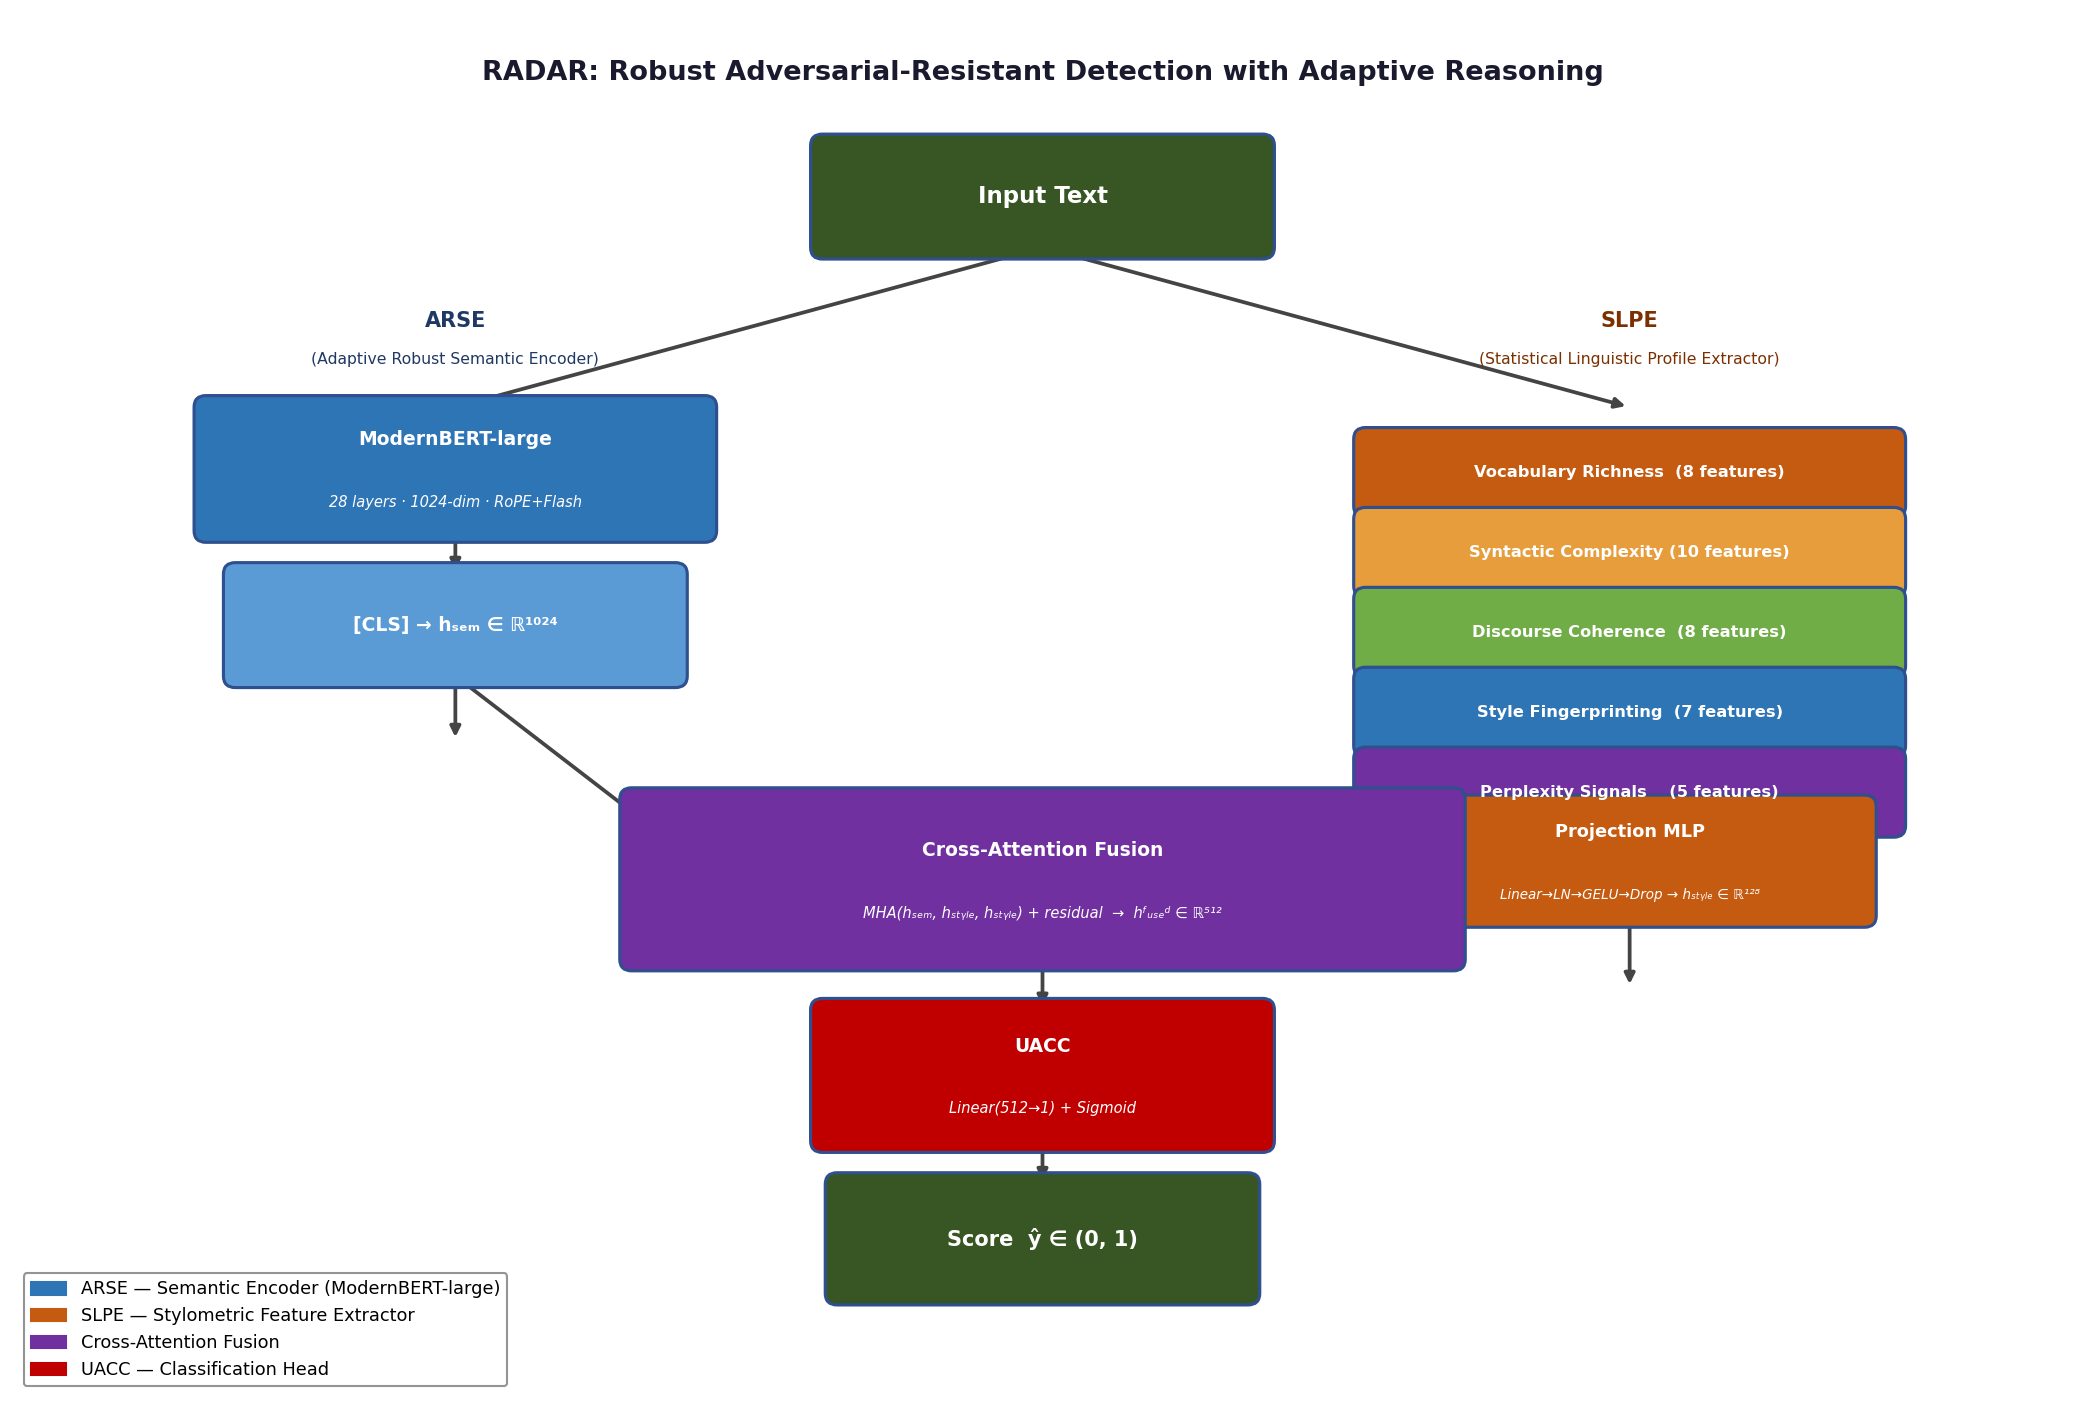
\includegraphics[width=\columnwidth]{images/radar_architecture.png}
  \caption{The RADAR architecture. Text enters two parallel pathways: the ARSE encoder
  extracts a contextual CLS embedding ($h_\text{semantic} \in \mathbb{R}^{1024}$) while the SLPE
  module computes a 38-dimensional stylometric feature vector. A cross-attention fusion layer
  integrates both representations into a unified embedding ($h_\text{fused} \in \mathbb{R}^{512}$),
  which is passed to the binary classifier.}
  \label{fig:radar_arch}
\end{figure}

\subsection{ARSE: Adaptive Reasoning Semantic Encoder}

The semantic encoding branch is built on \textbf{ModernBERT-large}~\cite{modernbert:2024}, a
bidirectional Transformer encoder with 28 attention layers, a hidden dimension of 1,024, and
395 million parameters. ModernBERT-large extends the classical BERT architecture with several
improvements relevant to long-document understanding: rotary positional embeddings (RoPE) for
improved extrapolation, alternating global and local attention patterns for computational
efficiency, and a context window of up to 8,192 tokens.

Given a text $x$, we tokenise with the ModernBERT tokeniser, truncating or padding to a maximum
sequence length of $L = 512$ tokens. The encoder processes the token sequence and produces a
sequence of contextual hidden states $\mathbf{H} \in \mathbb{R}^{L \times 1024}$. We extract the
CLS token representation $h_\text{semantic} = \mathbf{H}_{[0, :]} \in \mathbb{R}^{1024}$ as
the dense semantic summary of the input.

ModernBERT-large was selected over other encoders (e.g., RoBERTa-large, DeBERTa-v3-large) for
two reasons. First, its extended context window allows processing longer texts without aggressive
truncation, which is important for essays and news articles that constitute the PAN-2026 corpus.
Second, its training on code and scientific text in addition to web text provides broader
distributional coverage, which we hypothesise improves robustness to stylistic diversity.

\subsection{SLPE: Statistical Linguistic Profile Extractor}

\label{sec:slpe}

The stylometric branch extracts a 38-dimensional feature vector from the raw text, organised across
five linguistic categories. All features are normalised to the interval $[0, 1]$. The full feature
set is summarised in Table~\ref{tab:stylometric_features}.

\begin{table*}[t]
\caption{Summary of the 38 stylometric features extracted by the SLPE module, grouped by category.}
\label{tab:stylometric_features}
\begin{tabular}{lll}
\toprule
\textbf{Category} & \textbf{Features (\#)} & \textbf{Description} \\
\midrule
Vocabulary Richness   & 8 & TTR, Hapax ratio, Brunet's W, Honore's R, MATTR, TTR slope, \\
                      &   & Rare word ratio, Function word density \\
Syntactic Complexity  & 10 & Avg. sentence length, Sentence length variance, Clause density, \\
                      &    & Subordination ratio, Passive voice frequency, Noun phrase proxy, \\
                      &    & Verb density, Coordination frequency, Mean word position, Length skewness \\
Discourse Coherence   & 8 & Lexical cohesion (Jaccard), Pronoun density, Transition word frequency, \\
                      &   & Paragraph coherence (cosine), Topic consistency, Information flow variance, \\
                      &   & Semantic repetition ratio, Connective diversity \\
Style Fingerprinting  & 7 & Punctuation density, Capitalisation ratio, Number frequency, \\
                      &   & Quote usage, Parenthetical frequency, Paragraph length variance, List frequency \\
Perplexity Signals    & 5 & Forward entropy, Backward entropy, Entropy ratio, Burstiness, \\
                      &   & Mean surprisal \\
\midrule
\textbf{Total} & \textbf{38} & \\
\bottomrule
\end{tabular}
\end{table*}

\paragraph{Category 1 — Vocabulary Richness.} We compute eight features that quantify lexical
diversity: the Type-Token Ratio (TTR), the Hapax Legomena ratio, Brunet's~W~\cite{brunet:1978},
Honore's~R~\cite{honore:1979}, the Moving-Average TTR (MATTR) with a window of 100 tokens, the
slope of TTR across consecutive windows, the rare-word frequency, and the function-word density.
Together, these features characterise how diverse and distinctive the vocabulary is. Human writing
typically exhibits higher lexical diversity and a steeper TTR slope as the text progresses,
while LLM outputs tend toward greater lexical homogeneity~\cite{jakesch:2023}.

\paragraph{Category 2 — Syntactic Complexity.} Ten features characterise sentence-level structure:
average sentence length, sentence length variance, clause density (approximated via comma frequency),
subordination and coordination ratios, passive voice frequency (via a regex-based heuristic),
a noun-phrase proxy (mid-sentence capitalised tokens), verb density, mean relative word position
within sentences, and sentence length skewness. Research on AI-generated text has consistently found
that LLMs produce more uniform sentence lengths with lower variance~\cite{schuster:2020}, making
these features informative even under paraphrase attacks.

\paragraph{Category 3 — Discourse Coherence.} Eight features quantify text coherence at the
sentence and paragraph level: mean Jaccard similarity between adjacent sentences (lexical cohesion),
pronoun density, transition word frequency and diversity, paragraph-level cosine similarity
between adjacent paragraphs, topic consistency between the first and last paragraphs, information
flow regularity, and semantic repetition rate. Crucially, AI-generated text tends to exhibit
high local cohesion (smooth adjacency transitions) combined with lower global topic consistency,
a pattern that stylometric features can detect even when individual word choices are perturbed.

\paragraph{Category 4 — Style Fingerprinting.} Seven features capture surface-level authorial
fingerprints: punctuation density, capitalisation ratio, digit frequency, quote usage, parenthetical
frequency, paragraph length variance, and list structure frequency. While these features are the
easiest to alter through obfuscation, their combination with the more robust categories above
provides useful complementary signal.

\paragraph{Category 5 — Perplexity-Based Signals.} Five self-contained, LM-independent
features approximate perplexity-related signals using corpus statistics. We compute forward and
backward word-level entropy using the empirical unigram distribution of the text itself, their
ratio, the burstiness of information (variance in per-word surprisal values), and mean surprisal.
These features avoid the need for an external language model—a deliberate design choice that keeps
inference lightweight and avoids overfitting to a specific generator.

The extracted 38-dimensional vector is projected to 128 dimensions through a small MLP:
\begin{equation}
  h_\text{style} = \mathrm{GELU}(\mathrm{LayerNorm}(\mathbf{W}_s \mathbf{f}_\text{style} + \mathbf{b}_s)),
  \quad h_\text{style} \in \mathbb{R}^{128}
\end{equation}
where $\mathbf{f}_\text{style} \in \mathbb{R}^{38}$ is the raw feature vector and $\mathbf{W}_s$,
$\mathbf{b}_s$ are learned parameters.

\subsection{Cross-Attention Fusion Layer}

Naive concatenation of the semantic and stylometric representations would ignore the rich structural
relationship between the two modalities. Instead, RADAR uses a multi-head cross-attention mechanism
that allows the semantic representation to selectively query the stylometric representation,
learning which stylometric dimensions are most informative given the specific semantic content.

Formally, the projected style vector $h_\text{style} \in \mathbb{R}^{128}$ is first
linearly projected to match the semantic dimension:
\begin{equation}
  \tilde{h}_\text{style} = \mathbf{W}_{s2e}\, h_\text{style}, \quad \tilde{h}_\text{style} \in \mathbb{R}^{1024}
\end{equation}

Multi-head cross-attention is then applied with the semantic embedding as query and the
projected style vector as key and value:
\begin{equation}
  h_\text{attended} = \mathrm{MHA}\!\left(\underbrace{h_\text{semantic}}_{\text{query}},\;
  \underbrace{\tilde{h}_\text{style}}_{\text{key/value}}\right) + h_\text{semantic}
\end{equation}
followed by layer normalisation. The attention uses 8 heads. A residual connection is
applied to prevent information loss from the semantic branch.

Finally, the attended semantic representation is concatenated with the original
projected style vector and passed through a fusion MLP:
\begin{equation}
  h_\text{fused} = \mathrm{GELU}(\mathrm{LayerNorm}(\mathbf{W}_f\, [h_\text{attended};\, h_\text{style}] + \mathbf{b}_f)),
  \quad h_\text{fused} \in \mathbb{R}^{512}
\end{equation}
This two-level fusion—cross-attention followed by concatenation—ensures that the classifier
receives both the cross-modally attended information and the unmodified stylometric projection,
preventing the attention mechanism from wholly discarding fine-grained stylometric detail.

\subsection{UACC: Unified Authorship Classification Classifier}

The fused representation $h_\text{fused} \in \mathbb{R}^{512}$ is passed through a single
linear classifier to produce a scalar logit:
\begin{equation}
  z = \mathbf{w}_c^\top\, h_\text{fused} + b_c, \quad z \in \mathbb{R}
\end{equation}
The output confidence score is obtained via sigmoid activation:
\begin{equation}
  \hat{y} = \sigma(z) = \frac{1}{1 + e^{-z}}, \quad \hat{y} \in [0, 1]
\end{equation}
A score of $\hat{y} < 0.5$ indicates a human-authored text; $\hat{y} > 0.5$ indicates
AI-authored text; and $\hat{y} = 0.5$ is treated as ``undecidable'' in the PAN evaluation
framework.

\subsection{Loss Function and Class Imbalance}

Training uses binary cross-entropy with logits. The PAN-2026 training split contains
approximately 61.7\% AI-authored and 38.3\% human-authored samples, introducing a
class imbalance that can bias the model toward the majority class. To compensate, we
apply a positive-class weight $w_+ = N_\text{neg} / N_\text{pos}$, where
$N_\text{neg}$ and $N_\text{pos}$ are the number of human and AI samples respectively.
For our combined training set this yields $w_+ \approx 0.746$, i.e.~machine-authored
samples are down-weighted relative to human-authored samples, encouraging the model
to maintain balanced recall.

\subsection{Parameter Count}

The total parameter count is approximately 399.7~million, the vast majority of which
resides in the ModernBERT-large encoder (395.4~million). The stylometric projection,
fusion, and classification head account for approximately 4.9~million trainable parameters
(1.2\% of the total). This modular separation is exploited in our two-stage training
curriculum described in Section~\ref{sec:experiments}.
